% !TEX TS-program = xelatex
% !BIB program = bibtex
% !TeX spellcheck = ru_RU

% About magic macroses see also
% https://tex.stackexchange.com/questions/78101/

% По умолчанию используется шрифт 14 размера. Если нужен 12-й шрифт, уберите опцию [14pt]
\documentclass[14pt, russian]{matmex-diploma-custom}

% !TeX spellcheck = ru_RU
% !TEX root = game_lodygin.tex
% Опциональные добавления используемых пакетов. Вполне может быть, что они вам не понадобятся, но в шаблоне приведены примеры их использования.
\usepackage{tikz} % Мощный пакет для создание рисунков, однако может очень сильно замедлять компиляцию
\usetikzlibrary{decorations.pathreplacing,calc,shapes,positioning,tikzmark}

% Библиотека для TikZ, которая генерирует отдельные файлы для каждого рисунка
% Позволяет ускорить компиляцию, однако имеет свои ограничения
% Например, ломает пример выделения кода в листинге из шаблона
% \usetikzlibrary{external}
% \tikzexternalize[prefix=figures/]

\newcounter{tmkcount}

\tikzset{
  use tikzmark/.style={
    remember picture,
    overlay,
    execute at end picture={
      \stepcounter{tmkcount}
    },
  },
  tikzmark suffix={-\thetmkcount}
}

\usepackage{booktabs} % Пакет для верстки "более книжных" таблиц, вполне годится для оформления результатов
% В шаблоне есть команда \multirowcell, которой нужен этот пакет.
\usepackage{multirow}
\usepackage{siunitx} % для таблиц с единицами измерений

\newcommand{\cd}[1]{\texttt{#1}}
\newcommand{\inbr}[1]{\left<#1\right>}

% Для названий стоит использовать \textsc{}
\newcommand{\OCaml}{\textsc{OCaml}}
\newcommand{\miniKanren}{\textsc{miniKanren}}
\newcommand{\BibTeX}{\textsc{BibTeX}}
\newcommand{\vsharp}{\textsc{V$\sharp$}}
\newcommand{\fsharp}{\textsc{F$\sharp$}}
\newcommand{\csharp}{\textsc{C$\sharp$}}
\newcommand{\GitHub}{\textsc{GitHub}}
\newcommand{\SMT}{\textsc{SMT}}

\newcolumntype{L}[1]{>{\raggedright\let\newline\\\arraybackslash\hspace{0pt}}m{#1}}
%\newcolumntype{C}[1]{>{\centering\let\newline\\\arraybackslash\hspace{0pt}}m{#1}}
\newcolumntype{R}[1]{>{\raggedleft\let\newline\\\arraybackslash\hspace{0pt}}m{#1}}

%  Команды и пакеты, не используемые в шаблоне, которые тем не менее могут быть полезными.

% \newcolumntype{Y}{>{\centering\arraybackslash}X}

% \usepackage{mathrsfs}

% \lstdefinelanguage{ocaml}{
% keywords={@type, function, fun, let, in, match, with, when, class, type,
% nonrec, object, method, of, rec, repeat, until, while, not, do, done, as, val, inherit, and,
% new, module, sig, deriving, datatype, struct, if, then, else, open, private, virtual, include, success, failure,
% lazy, assert, true, false, end},
% sensitive=true,
% commentstyle=\small\itshape\ttfamily,
% keywordstyle=\ttfamily\bfseries, %\underbar,
% identifierstyle=\ttfamily,
% basewidth={0.5em,0.5em},
% columns=fixed,
% fontadjust=true,
% literate={->}{{$\to$}}3 {===}{{$\equiv$}}1 {=/=}{{$\not\equiv$}}1 {|>}{{$\triangleright$}}3 {\\/}{{$\vee$}}2 {/\\}{{$\wedge$}}2 {>=}{{$\ge$}}1 {<=}{{$\le$}} 1,
% morecomment=[s]{(*}{*)}
% }

\definecolor{Gray}{gray}{0.85}
\newcolumntype{a}{>{\columncolor{Gray}}c}

\usepackage{import}
\usepackage{xifthen}
\usepackage{pdfpages}
\usepackage{transparent}

\newcommand{\incfig}[1]{%
    \def\svgwidth{\columnwidth}
    \import{./figures/}{#1.pdf_tex}
}


\usepackage{totcount}

\begin{document}
% TODO: Formatting
% !TeX spellcheck = ru_RU
% !TEX root = bfs_lodygin.tex

%% Если что-то забыли, при компиляции будут ошибки Undefined control sequence \my@title@<что забыли>@ru
%% Если англоязычная титульная страница не нужна, то ее можно просто удалить.
\filltitle{ru}{
    %% Актуально только для курсовых/практик. ВКР защищаются не на кафедре а в ГЭК по направлению,
    %%   и к моменту защиты вы будете уже не в группе.
    chair              = {Кафедра системного программирования},
    group              = {22.Б07-мм},
    %
    %% Макрос filltitle ненавидит пустые строки, поэтому обязателен хотя бы символ комментария на строке
    %% Актуально всем.
    title              = {Исследование производительности алгоритма обхода графов в ширину},
    %
    %% Здесь указывается тип работы. Возможные значения:
    %%   production - производственная практика;
    %%   coursework - отчёт по курсовой работе;
    %%   practice - отчёт по учебной практике;
    %%   prediploma - отчёт по преддипломной практике;
    %%   master - ВКР магистра;
    %%   bachelor - ВКР бакалавра.
    type               = {practice},
    %
    %% Здесь указывается вид работы. От вида работы зависят критерии оценивания.
    %%   solution - <<Решение>>. Обучающемуся поручили найти способ решения проблемы в области разработки программного обеспечения или теоретической информатики с учётом набора ограничений.
    %%   experiment - <<Эксперимент>>. Обучающемуся поручили изучить возможности, достоинства и недостатки новой технологии, платформы, языка и т. д. на примере какой-то задачи.
    %%   production - <<Производственное задание>>. Автору поручили реализовать потенциально полезное программное обеспечение.
    %%   comparison - <<Сравнение>>. Обучающемуся поручили сравнить несколько существующих продуктов и/или подходов.
    %%   theoretical - <<Теоретическое исследование>>. Автору поручили доказать какое-то утверждение, исследовать свойства алгоритма и т.п., при этом не требуя написания кода.
    kind               = {experiment},
    %
    author             = {Лодыгин Леонид Александрович},
    %
    %% Актуально только для ВКР. Указывается код и название направления подготовки. Типичные примеры:
    %%   02.03.03 <<Математическое обеспечение и администрирование информационных систем>>
    %%   02.04.03 <<Математическое обеспечение и администрирование информационных систем>>
    %%   09.03.04 <<Программная инженерия>>
    %%   09.04.04 <<Программная инженерия>>
    %% Те, что с 03 в середине --- бакалавриат, с 04 --- магистратура.
    specialty          = {02.03.03 <<Математическое обеспечение и администрирование информационных систем>>},
    %
    %% Актуально только для ВКР. Указывается шифр и название образовательной программы. Типичные примеры:
    %%   СВ.5006.2017 <<Математическое обеспечение и администрирование информационных систем>>
    %%   СВ.5162.2020 <<Технологии программирования>>
    %%   СВ.5080.2017 <<Программная инженерия>>
    %%   ВМ.5665.2019 <<Математическое обеспечение и администрирование информационных систем>>
    %%   ВМ.5666.2019 <<Программная инженерия>>
    %% Шифр и название программы можно посмотреть в учебном плане, по которому вы учитесь.
    %% СВ.* --- бакалавриат, ВМ.* --- магистратура. В конце --- год поступления (не обязательно ваш, если вы были в академе/вылетали).
    programme          = {СВ.5006.2019 <<Математическое обеспечение и администрирование информационных систем>>},
    %
    %% Актуально только для ВКР, только для матобеса и только 2017-2018 годов поступления. Указывается профиль подготовки, на котором вы учитесь.
    %% Названия профилей можно найти в учебном плане в списке дисциплин по выбору. На каком именно вы, вам должны были сказать после второго курса (можно уточнить в студотделе).
    %% Вот возможные вариканты:
    %%   Математические основы информатики
    %%   Информационные системы и базы данных
    %%   Параллельное программирование
    %%   Системное программирование
    %%   Технология программирования
    %%   Администрирование информационных систем
    %%   Реинжиниринг программного обеспечения
    % profile            = {Системное программирование},
    %
    %% Актуально всем.
    %supervisorPosition = {проф. каф. СП, д.ф.-м.н., проф.}, % Терехов А.Н.
    supervisorPosition = {доцент кафедры информатики, к.~ф.-м.~н.,}, % Григорьев С.В.
    supervisor         = {С.~В.~Григорьев},
    %
    %% Актуально только для практик и курсовых. Если консультанта нет, закомментировать или удалить вовсе.
    %consultantPosition = {должность ООО <<Место работы>>, степень,},
    %consultant         = {К.~К.~Консультант},
    %
    %% Актуально только для ВКР.
    %reviewerPosition   = {должность ООО <<Место работы>> степень},
    %reviewer           = {Р.~Р.~Рецензент},
}

% \filltitle{en}{
%     chair              = {Advisor's chair},
%     group              = {ХХ.BХХ-mm},
%     title              = {Template for SPbU qualification works},
%     type               = {practice},
%     author             = {FirstName Surname},
%     %
%     %% Possible choices:
%     %%   02.03.03 <<Software and Administration of Information Systems>>
%     %%   02.04.03 <<Software and Administration of Information Systems>>
%     %%   09.03.04 <<Software Engineering>>
%     %%   09.04.04 <<Software Engineering>>
%     %% Те, что с 03 в середине --- бакалавриат, с 04 --- магистратура.
%     specialty          = {02.03.03 ``Software and Administration of Information Systems''},
%     %
%     %% Possible choices:
%     %%   СВ.5006.2017 <<Software and Administration of Information Systems>>
%     %%   СВ.5162.2020 <<Programming Technologies>>
%     %%   СВ.5080.2017 <<Software Engineering>>
%     %%   ВМ.5665.2019 <<Software and Administration of Information Systems>>
%     %%   ВМ.5666.2019 <<Software Engineering>>
%     programme          = {СВ.5006.2019 ``Software and Administration of Information Systems''},
%     %
%     %% Possible choices:
%     %%   Mathematical Foundations of Informatics
%     %%   Information Systems and Databases
%     %%   Parallel Programming
%     %%   System Programming
%     %%   Programming Technology
%     %%   Information Systems Administration
%     %%   Software Reengineering
%     % profile            = {Software Engineering},
%     %
%     %% Note that common title translations are:
%     %%   кандидат наук --- C.Sc. (NOT Ph.D.)
%     %%   доктор ... наук --- Sc.D.
%     %%   доцент --- docent (NOT assistant/associate prof.)
%     %%   профессор --- prof.
%     supervisorPosition = {Sc.D, prof.},
%     supervisor         = {S.S. Supervisor},
%     %
%     consultantPosition = {position at ``Company'', degree if present},
%     consultant         = {C.C. Consultant},
%     %
%     reviewerPosition   = {position at ``Company'', degree if present},
%     reviewer           = {R.R. Reviewer},
% }

\maketitle
\setcounter{tocdepth}{2}
\tableofcontents

% !TeX spellcheck = ru_RU
% !TEX root = bfs_lodygin.tex

\section*{Введение}
\thispagestyle{withCompileDate}

%В настоящее время одним из наиболее востребовательных методов для абстракции реальных систем является %представление этой системы в виде графа.
В настоящее время использование такой структуры данных как \textit{граф} имеет широкое применение для абстракции реальных систем с целью их дальнейшего анализа и обработки. Граф представляет из себя совокупность двух множеств --- объектов, называемых вершинами графа, и рёбер, обозначающих попарные связи между объектами. Такое представление используется в социальных науках , физике, химии, но чаще всего в информатике и сетевых технологиях, например, для хранения моделей машинного обучения, для работы с картами или же для хранения и обработки баз данных.

Для хранения графа в памяти используются различные представления, зависящие от соотношения количества вершин и рёбер в графе. К примеру, граф с относительно большим количеством рёбер часто представляется как \textit{матрица смежности}, где каждый столбец и строка обозначают вершину, а в ячейках хранится информация о наличии связи между данными вершинами. Становится очевидно, что в случае малого количества связей между вершинами, то есть когда исследуется \textit{разреженный граф}, такой подход для хранения не является рациональным, поэтому для оптимизации занимаемой памяти граф можно представить в виде \textit{дерева квадрантов}.

Графовая модель позволяет решать внушительный спектр задач, связанный с отношением между вершинами в графе. Для этого разработано большое количество алгоритмов, одним из которых является алгоритм обхода графа в ширину, иначе \textit{Breadth-first search}. При реализации такого алгоритма возможно применение \textit{векторно-матричных} операций, что позволяет естественным образом использовать \textit{многопоточное программирование} для оптимизации скорости работы алгоритма.

Общее количество вершин и \textit{плотность графа} непосредственно влияют на скорость работы алгоритма обхода в ширину, поэтому важной задачей является не только разработка параллельной версии такого алгоритма, но и исследование влияния этих параметров на его работу. 

% !TeX spellcheck = ru_RU
% !TEX root = game_lodygin.tex

\section{Постановка задачи}
\label{sec:task}
Целью данной работы является изучение возможностей игрового движка Unity путем командной разработки 3D игры в жанре survival horror. Для её выполнения были поставлены следующие задачи:

 \begin{enumerate}
 \item  Разработать концепт игры;
 \item  Провести обзор игр аналогичного жанра;
 \item  Изучить документацию Unity Engine;
 \item  Разработать следующие игровые механики:
   \begin{itemize}
   \item  передвижение игрока;
   \item  оружие и его анимации;
   \item  система психического состояния игрока;
   \item  система способностей игрока.
   \end{itemize}
 \item  Провести апробацию реализованных механик.
 \end{enumerate}

 Концепт игры разрабатывался с участием Плоскарева В.В, затем он приступил к отдельной задаче по реализации системы искуственного интеллекта для противников.

% !TeX spellcheck = ru_RU
% !TEX root = vkr.tex

\section{Обзор}
\label{sec:relatedworks}
Для реализации алгоритма и необходимых для его работы компонентов не лишним будет для начала рассмотреть базовую теорию графов, ознакомиться с существующими методами хранения больших данных в памяти и иметь представление о многопоточном программировании.

\subsection{Терминология}
\textit{Граф} $\mathcal{G} = \langle V, E \rangle$~--- упорядоченная пара множеств, где $V$ конечное непустое множество вершин графа, а $E \subseteq V \times V$ множество рёбер. Рёбра графа могут обладать дополнительной информацией, в таком случае граф называется \textit{взвешенным} и определятся тройкой $\langle V, E, L \rangle$, где $L$ это конечное множество меток графа. Под меткой стоит понимать данные, которые может содержать ребро в конкретной задаче. Например, если с помощью графа представлена карта, где города это вершины графа, а рёбра~--- дороги между городами, то в качестве меток могут быть взяты длины этих дорог.

\textit{Разреженный граф}~--- граф с малым количеством рёбер по отношению к количеству вершин.

Граф можно представлять в памяти как \textit{матрицу смежности}~--- квадратная матрица $M$ размеров $n \times n$, где $n$ это количество вершин в графе. Элементы такой матрицы $M[i,j]$ соответствуют единице, если между вершинами $i$ и $j$ существует ребро и нулю, если такое ребро отсутствует. В случае взвешенного графа, элементы матрицы принимают вместо единицы значение метки, соответствующее данному ребру.

\textit{Список рёбер}~--- другой подход к представлению графа в памяти. В списке рёбер в каждой строке записываются две смежные вершины и вес соединяющего 
их ребра (для взвешенного графа).

\textit{Путь}~--- это последовательность вершин и рёбер, в которой каждый элемент инцидентен предыдущему и последующему.

Две вершины в графе считаются \textit{связными}, если между ними существует путь.

\textit{Дерево}~---  ацикличный связный граф. Множество вершин в данном случае принято называть узлами, а множество рёбер~--- ветвями. Один узел дерева является \textit{корнем}, и он не имеет родителей. Все остальные узлы являются потомками корня. \textit{Листья}~--- это узлы дерева, которые не имеют потомков. Они находятся на самом нижнем уровне дерева.

\textit{Бинарное дерево}~---  это особый тип дерева, где каждый узел может иметь не более двух дочерних узлов.

\textit{Дерево квадрантов}~--- это дерево, в котором у каждого внутреннего узла ровно 4 потомка. Деревья квадрантов часто используются для рекурсивного разбиения двухмерного пространства по 4 квадранта (области).

\subsection{Представление графа в памяти}
Для хранения графа в памяти обычно используют матрицу смежности или список рёбер. При использовании матриц смежности в памяти создается двумерный массив, каждая ячейка которого соответствует элементу матрицы. Однако в случае малого количества рёбер в графе, такой подход нельзя считать рациональным, так как выделенная под несуществующие рёбра память расходуется впустую. При использовании списка рёбер проблема с избыточным использованием памяти решается, но возникают другие трудности, например, с добавлением новых рёбер или же с исследованием вершин на связность. Существует схожий со списком рёбер способ хранения в формате сжатой разреженной строки (\texttt{Compressed sparse row}), где матрица представляется тремя одномерными массивами, содержащими ненулевые значения, экстенты строк и индексы столбцов. Такой формат позволяет быстро обращаться к элементу по индексу и производить векторно-матричные операции, однако любое изменение графа в таком формате понесёт за собой большие накладные расходы, о чём говорится в статье Аапо Кироло~\cite{10.5555/2387880.2387884}.

Одним из решений данной проблем с избыточным использованием памяти является представление такой матрицы в виде дерева квадрантов, о чём в своей работе упоминает Гилберт~Дж.~Р.~\cite{bulucc2012parallel}. При таком подходе матрица рекурсивно разбивается на 4 части. В тот момент, когда в одной из частей отсутствуют значащие ячейки, разбиение останавливается и вся часть обозначается как незначащая. Преимуществом такой абстракции является не только сокращение объема памяти, требуемое для хранения графа, но и сохранение возможности применения векторно-матричных операций для реализации необходимых алгоритмов.

\subsection{Breadth-first search}
Обход в ширину~—-- один из простейших алгоритмов обхода графа, являющийся основой для многих важных алгоритмов для работы с графами. Он подразумевает поуровневое исследование графа:
\begin{enumerate}
\item  посещение одной или нескольких произвольно выбранных вершин;
\item  рекурсивное посещение всех смежных вершин для данной или данных.
\end{enumerate}
Вершины просматриваются в порядке возрастания кратчайшего пути до заданной. Алгоритм прекращает свою работу в случае обхода всех возможных вершин, либо в случае выполнения требуемого условия. Например, если задачей был поиск кратчайшего пути до определённой вершины. 

Данный алгоритм применяется для решения многих задач, одни из которых:
\begin{enumerate}
    \item  поиск кратчайшего пути;
    \item  поиск компонент связности;
    \item  поиск всех вершин/рёбер, лежащих на кратчайшем пути.
\end{enumerate}

Простейшей реализацией такого алгоритма является применение \textit{очереди}~--- абстрактного типа данных с дисциплиной доступа к элементам \enquote{первый пришёл --— первый вышел}. Первая вершина помещается в очередь с меткой $0$. Далее, рассматриваются все не посещенные ранее вершины, смежные с ней и добавляются в очередь с меткой данного шага алгоритма. Первая вершина удаляется из очереди и отмечается посещенной. Алгоритм продолжает работу, пока очередь не окажется пустой. Однако, существует другой подход к реализации данного алгоритма. Если граф представлен в виде матрицы смежности или же, в данном случае, в виде дерева квадрантов, такой алгоритм возможно реализовать с помощью векторно-матричных операций линейной алгебры~\cite{davis2018algorithm}. 

Тогда алгоритм будет выглядеть следующим образом.
\begin{enumerate}
    \item  На вход поступает матрица смежности графа и вектор, в ячейках которого отмечены стартовые вершины.
    \item  Вектор умножается на матрицу с помощью поэлементных операций и на выходе получается вектор, в ячейках которого отмечены вершины, смежные с изначальными.
    \item  Из данного вектора убираются все вершины, посещенные ранее.
    \item  Алгоритм завершает работу, когда вектор становится пустым.
\end{enumerate}

\subsection{Многопоточность}

\textit{Многопоточность}~--- это концепция, связанная с одновременным выполнением нескольких \textit{потоков} или нитей внутри одной программы. Потоки представляют собой последовательности инструкций, выполняющихся параллельно и независимо друг от друга, имея доступ к общим ресурсам программы. Многопоточные программы могут эффективно использовать многоядерные и многопроцессорные системы, что позволяет выполнять задачи параллельно и ускоряет выполнение программы. Однако такая концепция влечёт за собой ряд проблем. Во-первых, создание отдельного потока требует определённых ресурсов системы. При неумелом выделении количества потоков на решение задачи возможна потеря производительности, если накладные расходы на создание и \textit{синхронизацию} потоков превысят полученную выгоду от многопоточности. Во-вторых, при использовании общих ресурсов возникает риск \textit{состояния гонки} (race condition), когда несколько потоков пытаются одновременно изменять одни и те же данные. Это может привести к непредсказуемым результатам и ошибкам в программе. Наконец, многопоточность напрямую зависит от системы и её аппаратных возможностей. Количество \textit{ядер} и \textit{логических потоков} процессора однозначно определяют максимальное количество нитей, на которые следует разбивать нашу задачу во избежание потери производительности~\cite{Roberts2006MultiCorePI}.
%В обзоре необходимо ссылаться на работы других людей. В данном шаблоне задумано, что литература будет указываться в файле \verb=vkr.bib=. В нём указываются пункты литературы в формате \BibTeX{}, а затем на них можно ссылаться с помощью \verb=\cite{...}=. Та литература, на которую Вы сошлетесь, попадет в список литературы в конце документа. Если не сошлетесь~---  не попадёт. Спецификацию в формате \BibTeX{} почти никогда (для второго курса~--- никогда), не нужно придумывать руками. Правильно: находить в интернете описание цитируемой статьи\footnote{Например, \url{https://dl.acm.org/doi/10.1145/3408995} (дата доступа:   \DTMdate{2022-12-17}).},
%копировать цитату с помощью кнопки \foreignquote{english}{Export Citation} и вставлять в \BibTeX{} файл. Если так не делать, но оформление литературы будет обрастать багами.
%Например, \BibTeX{} по особенному обрабатывает точ\-ки, запятые и \verb=and= в списке авторов, что позволяет ему самому понимать, сколько авторов у статьи, и что там фамилия, что~--- имя, а что~--- отчество.

%В обзоре и в остальном тексте вы наверняка будете использовать названия продуктов или языков программирования. Для них рекоменду\-ется (в файле \verb=preamble2.tex=) за\-дать специальные команды, чтобы писать сложные названия правильно и одинаково по всему доку\-менту. Написать с ошибкой  название любимого языка программирова\-ния науч\-ного руко\-водителя~--- идеальный вариант его выбесить.

% !TeX spellcheck = ru_RU
% !TEX root = bfs_lodygin.tex

\section{Детали реализации}
В данном разделе предлагается рассмотреть основные детали реализации типов \texttt{SparseMatrix}, \texttt{SparseVector} и \texttt{Graph} для представления графов, а также реализацию векторно-матричных операций над этими типами и алгоритма \texttt{Breadth-first search} на основе этих операций. Разработка осуществлена на языке \fsharp. Полный код реализации доступен в публичном репозитории\footnote{Репозиторий с реализацией алгоритма:\url{https://github.com/LeonidLodygin/SPBU.2022.FunctionalProgramming.Homeworks} (дата доступа:   \DTMdate{2023-05-21}).}.

\subsection{SparseMatrix и SparseVector}
Тип \texttt{SparseVector} (листинг~\ref{sparsevector}) представляет из себя структуру данных, с которой возможны операции как с обычным массивом, например, обращение к элементу, но в то же время хранящуюся в памяти как тип \texttt{BinaryTree} (бинарное дерево, листинг~\ref{binarytree}). Такая реализация обусловлена оптимизацией выделения памяти под хранение экземпляров данного типа. Элементы вектора, обёрнутые в тип \textbf{Option} из библиотеки \textbf{Microsoft.FSharp.Core}, хранятся в листьях дерева. В том случае, если оба листа одного родителя пусты и обозначены как \texttt{None}, то листья \enquote{отрезаются} и родитель заменятся на \texttt{None}. Таким образом, векторы малой плотности будут занимать меньше памяти для хранения, чем такие же векторы, представленные в памяти в виде обычного массива, но в то же время будут сохранять все свойства векторов.

\lstdefinestyle{codelistingstyle}{
    backgroundcolor=\color{white},   
    commentstyle=\color{green},
    keywordstyle=\color{magenta},
    numberstyle=\tiny\color{gray},
    stringstyle=\color{purple},
    basicstyle=\ttfamily\footnotesize,
    breakatwhitespace=false,         
    breaklines=true,                                     
    keepspaces=true,                 
    numbers=left,                    
    numbersep=5pt,                  
    showspaces=false,                
    showstringspaces=false,
    showtabs=false,                  
    tabsize=2
}

\begin{lstlisting}[style=codelistingstyle, caption={Тип SparseVector},label={sparsevector}, frame=single]
type SparseVector<'Value when 'Value: equality> =
    val Memory: BinaryTree<'Value>
    val Length: uint
\end{lstlisting}

\begin{lstlisting}[style=codelistingstyle, caption={Тип BinaryTree},label={binarytree}, frame=single]
type BinaryTree<'Value> =
    | Node of BinaryTree<'Value> * BinaryTree<'Value>
    | Leaf of 'Value
    | None
\end{lstlisting}

Для сложения экземпляров типа \texttt{SparseVector} реализована функция \texttt{ParallelFAddVector}, принимающая два вектора одинакового размера и возвращающая результирующий вектор, в ячейках которого лежат результаты поэлементной операции, переданной в качестве вспомогательной функции. \texttt{ParallelFAddVector} с помощью рекурсивной функции \texttt{helper} обходит оба дерева и, доходя до листьев, применяет необходимую операцию к значениям в листьях. Пример вспомогательной функции для математического сложения векторов в листинге~\ref{helpfunc} 

\begin{lstlisting}[style=codelistingstyle, caption={Пример вспомогательной поэлементной функции},label={helpfunc}, frame=single]
let fAdd a b =
    match a, b with
    | Some x, Some y ->
        if x + y <> 0 then
            Some(x + y)
        else
            Option.None
    | Option.None, Some x -> Some x
    | Some x, Option.None -> Some x
    | Option.None, Option.None -> Option.None
\end{lstlisting}

Представление в виде двоичных деревьев сохраняет возможность использования многопоточности при реализации такой функции. Для сложения векторов необходимо рекурсивно обходить оба дерева, представляющие данные векторы, и, доходя до листьев, соответствующих ячейкам в векторах с одинаковым индексом, применять к ним поэлементную операцию. Функция для обхода деревьев на каждом шаге сопоставляет узлы деревьев. В том случае, если оба узла имеют по два дочерних, не отмеченных как \texttt{None} узла, происходит два рекурсивных вызова функции от дочерних узлов, следовательно, в данном месте имеется возможность для использования параллельных вычислений (листинг~\ref{addparallel}). Для контроля количества потоков в функцию \texttt{ParallelFAddVector} передается параметр типа \texttt{int}, определяющий количество потоков в степени двойки, которое мы хотим выделить для работы функции.

\begin{lstlisting}[style=codelistingstyle, caption={Разделение задачи сложения двух деревьев на две подзадачи и использование потоков для получения результата},label={addparallel}, frame=single]
| Node (left, right), Node (left2, right2) ->
    if level = 0 then
        Node(helper left left2 level, helper right right2 level)
        |> NoneDestroyer
    else
        let tasks =
            [| async { return helper left left2 (level - 1) }
               async { return helper right right2 (level - 1) } |]

        let results = tasks |> Async.Parallel |> Async.RunSynchronously
        Node(results[0], results[1]) |> NoneDestroyer
\end{lstlisting}

Объекты типа \texttt{SparseMatrix} аналагично объектам типа \texttt{SparseVector} хранятся в памяти в виде дерева квадрантов. Абстракция позволяет взаимодействовать с такими объектами как с двумерными массивами и, соответственно, применять к ним векторно-матричные операции. Для умножения вектора типа \texttt{SparseVector} на матрицу типа \texttt{SparseMatrix} была реализована функция \texttt{ParallelMultiplyVecMat}, принимающая вектор, матрицу и возращающая результирующий вектор. Аналогично функции сложения, данная функция легко поддается разделению на подзадачи для параллельных вычислений. Входной параметр \texttt{parallelLevel} определяет количество подзадач в четвёртой степени.

\subsection{Breadth-first search}
Функция \texttt{Bfs} принимает на вход объект типа \texttt{Graph} (листинг~\ref{graph}), хранящийся в памяти как \texttt{SparseMatrix}, список стартовых вершин и два числовых параметра, отвечающих за многопоточность --- \texttt{fAddLevel}, который затем передаётся в функцию сложения векторов и \texttt{multLevel}, передающийся функции умножения(листинг~\ref{bfs}).

\newpage
\begin{lstlisting}[style=codelistingstyle,caption={Тип Graph},label={graph}, frame=single]
type Graph<'Value when 'Value: equality> =
    val Memory: SparseMatrix<'Value>
    val Vertices: uint
    val Edges: uint
\end{lstlisting}

\begin{lstlisting}[style=codelistingstyle, caption={Алгоритм Bfs с использованием векторно-матричных операций},label={bfs}, frame=single]
let Bfs (graph: Graph<'Value>) (apexes: List<uint>) fAddLevel multLevel =
    let apexes = List.map (fun x -> (x, ())) apexes
    let front = SparseVector(apexes, graph.Vertices)

    let visited =
        ParallelFAddVector(SuperSum 0u) 
            front 
            (SparseVector(BinaryTree.None, graph.Vertices)) fAddLevel

    let rec helper (front: SparseVector<'A>) visited iter =
        if front.IsEmpty then
            visited
        else
            let newFront =
                ParallelFAddVector
                    Mask
                    (ParallelMultiplyVecMat front graph.Memory FrontAdd FrontMult multLevel)
                    visited
                    fAddLevel

            let visited = ParallelFAddVector(SuperSum iter) newFront visited fAddLevel
            helper newFront visited (iter + 1u)

    helper front visited 1u
\end{lstlisting}

По данном списку создается вектор \texttt{front}, который на каждом шаге алгоритма будет содержать актуальные вершины, в которых мы находимся. Далее, создается вектор посещенных уже ранее вершин с помощью функции сложения векторов и вспомогательной поэлементной функции \texttt{SuperSum} (листинг~\ref{supersum}). 

Далее, запускается вспомогательная рекурсивная функция, которая будет умножать \texttt{front} на матрицу, убирать из него уже посещенные ранее вершины с помощью поэлементной функции \texttt{Mask} (листинг~\ref{mask}) и складывать новые посещенные вершины в вектор посещенных вершин. Алгоритм завершает свою работу, когда \texttt{front} становится пустым. 

\begin{lstlisting}[style=codelistingstyle, caption={Вспомогательная поэлементная функция для определения посещенных вершин},label={supersum}, frame=single]
let SuperSum iter value1 value2 =
    match value1, value2 with
    | Option.None, Option.None -> Option.None
    | Option.None, value2 -> value2
    | Some _, Option.None -> Some iter
\end{lstlisting} 

\begin{lstlisting}[style=codelistingstyle, caption={Вспомогательная поэлементная функция для удаления из ветора front посещенных ранее вершин},label={mask}, frame=single]
let Mask value1 value2 =
    match value1, value2 with
    | Option.None, _ -> Option.None
    | Some value1, Option.None -> Some value1
    | Some _, _ -> Option.None
\end{lstlisting}
% !TeX spellcheck = ru_RU
% !TEX root = bfs_lodygin.tex

\section{Эксперимент}

В данном разделе предлагается рассмотреть результаты экспериментального исследования реализованного алгоритма обхода графа в ширину. Основная задача: выявить зависимость производительности алгоритма от входных параметров графа и количества асинхронных потоков, обрабатывающих данный алгоритм.

\subsection{Условия эксперимента}
Для экспериментов использовалась рабочая станция с процессором Intel Core i5-10300H с тактовой частотой 2.50GHz, RAM DDR4 объемом 8гб под управлением OC Windows 10.

\subsection{Исследовательские вопросы }

\begin{itemize}
\item[\textbf{RQ1:}] При каких параметрах графа выгоднее использовать параллельную версию алгоритма, а при каких последовательную?
\item[\textbf{RQ2:}] Использование какого количества потоков даёт наибольший выигрыш в производительности и почему?
\end{itemize}


\subsection{Метрики}
В качестве метрик производительности используется время, требуемое на завершение алгоритма. Показатели времени получены с помощью библиотеки \texttt{BenchmarkDotNet v0.13.5}\footnote{Репозиторий библиотеки \texttt{BenchmarkDotNet}: \url{https://github.com/dotnet/BenchmarkDotNet} (дата доступа:   \DTMdate{2023-05-21}).}. Для замеров были выбраны стандартные настройки по \enquote{прогреву} и количеству итераций для измерений.

Для анализа алгоритма было решено воспользоваться собственным генератором графов нужного размера с нужной плотностью. Данный подход позволяет минимизировать влияние разницы прочих параметров на исследуемый, следовательно результаты, полученные в таком исследовании, позволят точнее выявить необходимые зависимости, нежели при использовании уже существующих графов. Генератор принимает на вход количество вершин в графе и параметр \texttt{density} типа \texttt{float}, отвечающий за плотность графа. По количеству заданных вершин создаётся двумерный массив, ячейки которого заполняются следующим образом. Если параметр плотности графа меньше $0.5$, все ячейки массива заполняются \texttt{Option.None}, затем с помощью цикла в случайных ячейки массива заносятся сгенерированные случайные числа \texttt{int}, обёрнутые в тип \texttt{Option}, пока не будет достигнута необходимая плотность. В противном случае, массив полностью заполняется случайными числами типа \texttt{int}, обёрнутыми в тип \texttt{Option}, а в случайные ячейки заносятся \texttt{Option.None}, пока опять же таки не будет достигнута необходимая плотность. 

\subsection{Результаты}

Входные параметры:
 \begin{enumerate}
 \item  \texttt{Vertices} --- количество вершин в графе; 
 \item  \texttt{Density} --- плотность графа;
 \item \texttt{parallelMult} --- уровень распараллеливания функции умножения, каждый уровень увеличивает число подзадач в 4 раза;
  \item \texttt{parallelAdd} --- уровень распараллеливания функции сложения, каждый уровень увеличивает число подзадач в 2 раза.
\end{enumerate}

Результаты замеров:
\begin{enumerate}
\item  \texttt{Time} --- результат измерений в мс (за исключением таблицы~\ref{bfscomparison}, где время измерений указано в микросекундах и таблицы~\ref{bfsmaxgraph}, где время указано в секундах);
\end{enumerate}

Замеры проводились начиная от очень малых графов (10 вершин), заканчивая графами с 5000 вершинами. Дополнительно были исследованы графы с 10000 вершинами, но очень малой плотности. Выбор максимального размера графа связан с ограничением оперативной памяти системы, на которой производились вычисления.

В таблице~\ref{bfs0} представлены результаты замеров времени работы последовательного алгоритма при различных входных параметрах графа. Из данной таблицы видно, что время работы алгоритма возрастает с увеличением плотности графа, а затем, когда граф достигает плотности $0.5$ начинает снижаться. Не трудно догадаться, что при высокой плотности графа уменьшается количество шагов алгоритма, необходимых для его завершения, так как за каждый шаг будет осуществляться переход в большее количество смежных вершин, следовательно общее время работы уменьшается.

\begin{table}[h]
\centering
    \caption{Производительность последовательного алгоритма обхода графов в ширину.}
    \rowcolors{2}{black!2}{black!10}
    \scalebox{0.7}{
    \begin{tabular}{| a | r | r | a | r | r |}
    \hline
        \textsc{Vertices} & \textsc{Density} & \textsc{Time} &
         \textsc{Vertices} & \textsc{Density} & \textsc{Time} \\ 
        \hline
        500 & 0.1 & $17 \pm 0.1$ & 2500 & 0.1 & $429 \pm 2$  \\ 
        500 & 0.3 & $33 \pm 0.3$ & 2500 & 0.3 & $860 \pm 3$ \\
        500 & 0.5 & $44 \pm 0.2$ & 2500 & 0.5 & $1091 \pm 8$ \\
        500 & 0.7 & $42 \pm 0.2$ & 2500 & 0.7 & $1095 \pm 3$  \\ 
        500 & 0.9 & $36 \pm 0.2$ & 2500 & 0.9 & $980 \pm 4$  \\ 
        
        1000 & 0.1 & $68 \pm 0.4$ & 5000 & 0.1 & $1717 \pm 3$ \\ 
        1000 & 0.3 & $137 \pm 0.6$ & 5000 & 0.3 & $3531 \pm 20$ \\
        1000 & 0.5 & $182 \pm 1.1$ & 5000 & 0.5 & $4426 \pm 23$ \\
        1000 & 0.7 & $179 \pm 1.2$ & 5000 & 0.7 & $4421 \pm 9$ \\ 
        1000 & 0.9 & $158 \pm 0.3$ & 5000 & 0.9 & $3984 \pm 14$ \\ 
    \hline    
    \end{tabular}%
    }
    \label{bfs0}
\end{table}

В таблице~\ref{bfsparallel} приведены результаты замеров времени работы параллельного алгоритма обхода графа при различных параметрах. Для удобства, при каждом параметре плотности графа взята наилучшая скорость среди всех параллельных версий алгоритма. Из полученных результатов можно заметить, что при увеличении размеров графа, наиболее оптимальное количество подзадач для параллельных вычислений выравнивается к 16 для функции умножения. Стоить отметить, что на достаточно больших графах, при одном и том же уровне распараллеливания функции умножения, влияние распараллеливания функции сложения становится не столь существенным, любая из комбинаций даёт один и тот же результат по времени в пределах погрешности (таблица~\ref{parallelAddvsparallelMult}). Связано это с тем, что наибольший процент времени выделяется под функцию умножения, как наиболее затратную по ресурсам.

\begin{table}[H]
\centering
    \caption{Производительность параллельного алгоритма обхода графов в ширину (лучшие данные по метрике). Графа \texttt{SpeedUp} показывает отношение скорости работы параллельной версии алгоритма к скорости работы последовательной версии. }
    \rowcolors{2}{black!2}{black!10}
    \scalebox{0.5}{
    \begin{tabular}{| a | r | r | r | r | r |}
    \hline
        \textsc{Vertices} & \textsc{Density} & \textsc{parallelMult} & \textsc{parallelAdd} & \textsc{SpeedUp}\\
        \hline
        500 & 0.1 & 2 & 1 & 0.53\\ 
        500 & 0.3 & 1 & 1 & 0.57\\ 
        500 & 0.5 & 1 & 1 & 0.56\\ 
        500 & 0.7 & 1 & 2 & 0.62\\
        500 & 0.9 & 2 & 2 & 0.64\\        
        1000 & 0.1 & 1 & 1 & 0.54\\ 
        1000 & 0.3 & 1 & 1 & 0.53\\ 
        1000 & 0.5 & 1 & 1 & 0.5\\
        1000 & 0.7 & 1 & 2 & 0.55\\ 
        1000 & 0.9 & 1 & 3 & 0.57\\ 
        2500 & 0.1 & 2 & 3 & 0.56 \\
        2500 & 0.3 & 2 & 3 & 0.54 \\
        2500 & 0.5 & 2 & 1 & 0.53 \\
        2500 & 0.7 & 2 & 3 & 0.59\\
        2500 & 0.9 & 2 & 1 & 0.6  \\ 
        5000 & 0.1 & 2 & 1 & 0.56 \\ 
        5000 & 0.3 & 2 & 3 & 0.51 \\
        5000 & 0.5 & 2 & 1 & 0.53 \\
        5000 & 0.7 & 2 & 3 & 0.59 \\ 
        5000 & 0.9 & 2 & 1 & 0.58 \\ 
    \hline    
    \end{tabular}%
    }
    \label{bfsparallel}
\end{table}

\begin{table}[h]
\centering
    \caption{Сравнение влияния уровня распараллеливания функции умножения и уровня распараллеливания функции сложения на графе с 5000 вершинами.}
    \rowcolors{2}{black!2}{black!10}
    \scalebox{0.7}{
    \begin{tabular}{| a | r | r | r | r |}
    \hline
        \textsc{Vertices} & \textsc{Density} & \textsc{parallelMult} & \textsc{parallelAdd} & \textsc{Time}\\ 
        \hline
        5000 & 0.1 & 1 & 1 & $1411 \pm 10$  \\ 
        5000 & 0.1 & 1 & 2 & $1401 \pm 12$  \\
        5000 & 0.1 & 1 & 3 & $1409 \pm 9$  \\
        5000 & 0.1 & 2 & 1 & $970 \pm 19$  \\
        5000 & 0.1 & 2 & 2 & $998 \pm 19$  \\
        5000 & 0.1 & 2 & 3 & $980 \pm 19$  \\
        5000 & 0.1 & 3 & 1 & $1126 \pm 21$  \\
        5000 & 0.1 & 3 & 2 & $1138 \pm 23$  \\
        5000 & 0.1 & 3 & 3 & $1151 \pm 18$  \\
    \hline    
    \end{tabular}%
    }
    \label{parallelAddvsparallelMult}
\end{table}


Так как на всех параметрах графа параллельная версия алгоритма обходила по производительности последовательную, было решено произвести дополнительные замеры при графах с меньшим количеством вершин (таблица~\ref{bfscomparison}). Выяснилось, что при таких размерах графа последовательная версия работает значительно быстрее, чем параллельная.

\begin{table}[h]
\centering
    \caption{Сравнение производительности параллельного и обычного Bfs на графах с 10 вершинами. Графа \texttt{SpeedUp} показывает отношение скорости работы параллельной версии алгоритма к скорости работы последовательной версии.}
    \rowcolors{2}{black!2}{black!10}
    \scalebox{0.7}{
    \begin{tabular}{| a | r | r | r | r |}
    \hline
        \textsc{Vertices} & \textsc{Density} & \textsc{TimeBfs} & \textsc{TimeParallelBfs} & \textsc{SpeedUp}\\
        \hline
        10 & 0.1 & $15.00 \pm 0.03$ & $53 \pm 0.2$ & 3.5 \\ 
        10 & 0.3 & $20 \pm 0.4$ & $78 \pm 0.3$ & 3.9 \\
        10 & 0.5 & $32 \pm 0.3$ & $124 \pm 1.3$ & 3.8 \\
        10 & 0.7 & $27 \pm 0.5$ & $60 \pm 0.4$ & 2.2 \\
        10 & 0.9 & $25 \pm 0.6$ & $44 \pm 0.4$ & 1.76\\ 
    \hline    
    \end{tabular}%
    }
    \label{bfscomparison}
\end{table}

Однако, уже на графах с 50 вершинами параллельная версия догоняет и начинает опережать последовательную версию по производительности.

\begin{table}[h]
\centering
    \caption{Сравнение производительности параллельного и обычного Bfs на графах с 50 вершинами. Графа \texttt{SpeedUp} показывает отношение скорости работы параллельной версии алгоритма к скорости работы последовательной версии.}
    \rowcolors{2}{black!2}{black!10}
    \scalebox{0.7}{
    \begin{tabular}{| a | r | r | r | r |}
    \hline
        \textsc{Vertices} & \textsc{Density} & \textsc{TimeBfs} & \textsc{TimeParallelBfs} & \textsc{SpeedUp}\\
        \hline
        50 & 0.1 & $293 \pm 6$ & $284 \pm 3$ & 0.97 \\ 
        50 & 0.3 & $372 \pm 7$ & $278 \pm 5$ & 0.74\\ 
        50 & 0.5 & $572 \pm 11$ & $614 \pm 9$ & 1.07\\
        50 & 0.7 & $438 \pm 7$ & $325 \pm 2$ & 0.74 \\
        50 & 0.9 & $416 \pm 8$ & $312 \pm 2$ & 0.75 \\ 
    \hline    
    \end{tabular}%
    }
    \label{bfscomparison}
\end{table}

Также, чтобы исследовать оптимальное разделение на подзадачи для функции умножения, как наиболее значимой для распараллеливания, были проведены замеры с теми же размерами и плотностями графа, но с использованием последовательной функции сложения. Результаты приведены в таблице~\ref{bfsparallelmult}.

\begin{table}[h]
\centering
    \caption{Производительность параллельного алгоритма обхода графов в ширину с использованием последовательной функции сложения веторов.}
    \rowcolors{2}{black!2}{black!10}
    \scalebox{0.6}{
    \begin{tabular}{| a | r | r | r | a | r | r | r |}
    \hline
        \textsc{Vertices} & \textsc{Density} & \textsc{parallelMult} & \textsc{Time} &
        \textsc{Vertices} & \textsc{Density} & \textsc{parallelMult} & \textsc{Time} \\ 
        \hline
        500 & 0.1 & 1 & $9,8 \pm 0.1$ & 2500 & 0.1 & 2 & $240 \pm 3$  \\ 
        500 & 0.3 & 1 & $19 \pm 0.4$ & 2500 & 0.3 & 2 & $470 \pm 9$ \\ 
        500 & 0.5 & 2 & $44 \pm 0.9$ & 2500 & 0.5 & 2 & $1004 \pm 19$ \\
        500 & 0.7 & 1 & $26 \pm 0.5$ & 2500 & 0.7 & 2 & $661 \pm 13$  \\
        500 & 0.9 & 2 & $24 \pm 0.4$ & 2500 & 0.9 & 2 & $620 \pm 12$  \\ 
        
        1000 & 0.1 & 1 & $36 \pm 0.5$ & 5000 & 0.1 & 2 & $923 \pm 18$ \\
        1000 & 0.3  & 1 & $72 \pm 1.4$ & 5000 & 0.3 & 2 & $1843 \pm 36$ \\
        1000 & 0.5  & 2 & $153 \pm 1.4$ & 5000 & 0.5 & 2 & $4143 \pm 78$ \\
        1000 & 0.7 & 1 & $98 \pm 1.6$ & 5000 & 0.7 & 2 & $2571 \pm 39$ \\ 
        1000 & 0.9 & 1 & $90 \pm 1.1$ & 5000 & 0.9 & 2 & $2372 \pm 41$ \\
    \hline    
    \end{tabular}%
    }
    \label{bfsparallelmult}
\end{table}

В ходе замеров было установлено, что при увеличении размеров графа, вне зависимости от плотности, время работы алгоритма при разделении на 16 подзадач для функции умножения хоть и больше, чем при работе с разделением на 64 подзадачи, но разрыв становится все меньше и меньше. Вследствие этого наблюдения, было решено произвести замеры для параллельных версий алгоритма для графов с 10000 вершинами, что являлось пределом допустимого значения количества вершин для обработки графа системой. Исследовались графы маленькой плотности с целью выяснить, сможет ли версия с 64 подзадачами обогнать по производительности версию с 16 подзадачами. Результаты приведены в таблице~\ref{bfsmaxgraph}.

\begin{table}[h]
\centering
    \caption{Сравнение производительности алгоритма обхода в ширину при распараллеливании на 16 и 64 подзадачи для функции умножения. Графа \texttt{SpeedUp} показывает отношение скорости работы алгоритма при 64 подзадачах к скорости работы при 16 подзадачах.}
    \rowcolors{2}{black!2}{black!10}
    \scalebox{0.6}{
    \begin{tabular}{| a | r | r | r | r | r |}
    \hline
        \textsc{Vertices} & \textsc{Density} & \textsc{parallelMult} & \textsc{Time} &
        \textsc{SpeedUp} \\ 
        \hline
        1000 & 0.1 & 2 & $0.0400 \pm 0.0003$ & 1.25 \\
        2500 & 0.1 & 2 & $0.240 \pm 0.002$ & 1.22 \\ 
        5000 & 0.1 & 2 & $0.9 \pm 0.03$ & 1.2 \\
        10000 & 0.1 & 2 & $4 \pm 0.07$ & 1.25 \\ 
    \hline    
    \end{tabular}%
    }
    \label{bfsmaxgraph}
\end{table}

Однако, как показало дополнительное измерение при графе с 10000 вершинами, по производительности всё так же лидирует распараллеливание на 16 подзадач, причём разрыв между скоростями вырос.

Результаты, полученные с помощью \texttt{BenchmarkDotNet} были проверены на адекватность с помощью библиотек \texttt{SciPy v1.10.1}\footnote{Сайт библиотеки \texttt{SciPy}: \url{https://scipy.org/} (дата доступа:   \DTMdate{2023-05-21}).}, \texttt{NumPy v1.24.3}\footnote{Сайт библиотеки \texttt{NumPy}: \url{https://numpy.org/} (дата доступа:\DTMdate{2023-05-21}).} и \texttt{Matplotlib v3.7.1}\footnote{Сайт библиотеки \texttt{MatPlotLib}: \url{https://matplotlib.org/} (дата доступа:   \DTMdate{2023-05-21}).} на языке \texttt{Python}. Например, рассмотрим данные, полученные при измерении производительности параллельной версии алгоритма на графе с 5000 вершинами плотности $0.9$ и уровнями распараллеливания parallelMult, равным двум, и parallelAdd, равным 1. Результаты замеров приведены в таблице~\ref{data}. 

\begin{table}[h]
\centering
    \caption{Замеры времени работы параллельной версии алгоритма на графе с 5000 вершинами плотности $0.9$. Функция умножения разделена на 16 подзадач, функция сложения на две. Время измерено в секундах.}
    \rowcolors{2}{black!2}{black!10}
    \scalebox{0.6}{
    \begin{tabular}{| a | r | r | r | r | r | r | r | r | r | r |}
    \hline
    N & 1 & 2 & 3 & 4 & 5 & 6 & 7 & 8 & 9 & 10 \\
    \hline
    Time & 2.4081 & 2.3506 & 2.3857 & 2.3383 & 2.2634 & 2.2931 & 2.2984 & 2.3895 & 2.2800 & 2.2899\\
    N & 11 & 12 & 13 & 14 & 15 & 16 & 17 & 18 & 19 & 20\\
    \hline
    Time & 2.3293 & 2.2977 & 2.2358 & 2.3113 & 2.4044 & 2.3317 & 2.3054 & 2.2614 & 2.4011 & 2.3421 \\
    \hline    
    \end{tabular}%
    }
    \label{data}
\end{table}

С помощью функций \texttt{scipy.stats.shapiro()} (тест Шапиро-Уилка) и \texttt{scipy.stats.normaltest()} (критерий согласия Пирсона) было проверено соответствие выборки нормальному распределению. Значение \texttt{pvalue} в результате проверок равнялось 0.36 (Шапиро) и 0.5 (Пирсон), что позволяет нам не отклонять \enquote{нулевую гипотезу} и считать полученные данные как нормальное распределение. Далее, с помощью функций \texttt{np.mean()} и \texttt{np.std()} были посчитаны среднее значение $Mean = 2.32586$ и стандартное отклонение $StdDev = 0.051$. Аналогичные результаты были получены и библиотекой \texttt{BenchmarkDotNet}: $Mean = 2.326$, $StdDev = 0.051$. При помощи \texttt{matplotlib.pyplot.hist()} была построена гистограмма (рисунок~\ref{fig:plot}) из полученной выборки.

\begin{figure}[H]
    \centering
    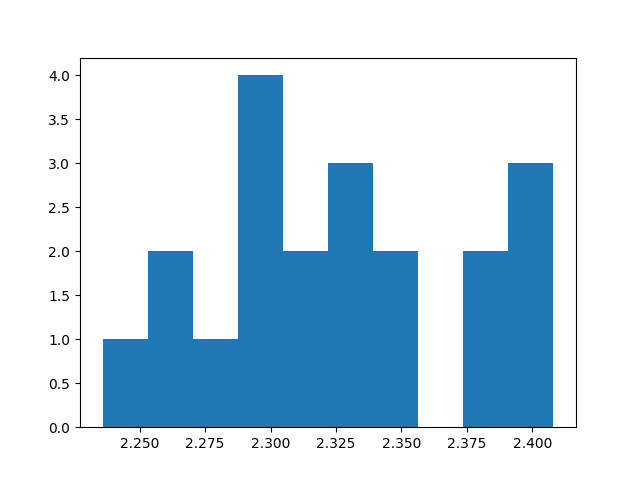
\includegraphics[width=\textwidth]{figures/plot.png}
    \caption{Гистограмма распределения данных}
    \label{fig:plot}
\end{figure}

\subsubsection{RQ1} Исходя из полученных данных, последовательная версия алгоритма работает быстрее параллельной только на очень малых графах (10 вершин), когда накладные расходы на выделение дополнительных потоков и их синхронизацию влияют сильнее, чем ускорение относительно последовательной версии. При входных графах от 50 вершин и более, параллельная версия даёт прирост к производительности вплоть до увеличения скорости работы алгоритма в 2 раза при любых параметрах плотности.
\subsubsection{RQ2} В ходе экспериментов было установлено, что использование разделения на 16 подзадач, начиная с определённых размеров графа (2500 вершин для системы, используемой при замерах), даёт максимальный прирост по производительности алгоритма обхода в ширину. Такой результат можно объяснить количеством ядер процессора. Система, на которой производились замеры имеет 4-х ядерный процессор \texttt{Intel Core i5-10300H}, вследствие чего количество независимых вычислителей равняется четырём. С другой стороны, данный процессор поддерживает технологию \texttt{Hyper-Threading}, позволяющую разделить одно ядро процессора на 2 отдельных логических процессора, работающих независимо. Таким образом наилучшая производительность наблюдается на 8 потоках, каждый из которых обрабатывает по 2 подзадачи. Польза от такого разделения влияет на конечное время работы алгоритма сильнее, чем затраты времени на выделение необходимых потоков и синхронизацию их работы.
% !TeX spellcheck = ru_RU
% !TEX root = game_lodygin.tex

\section*{Заключение}
В рамках проведения работы были получены следующие результаты.

\begin{itemize}
\item Разработан концепт игры.
\item Проведен обзор существующих аналогов.
\item Изучена документация используемого движка.
\item Реализована модель главного героя и некоторые игровые механики, такие как:
    \begin{enumerate}
       \item  Передвижение игрока;
       \item  Оружие и его анимации;
       \item  Система психического состояния игрока;
       \item  Система способностей игрока.
    \end{enumerate}   
\end{itemize}

\noindent В качестве будущих задач можно выделить следующие пункты.
\begin{itemize}
\item Расширение системы способностей игрока.
\item Реализация стрельбы и системы здоровья персонажа.
\item Система инвентаря.
\item Интерактивное окружение.
\item Расширение системы психического состояния персонажа.
\end{itemize}

Полный код реализации доступен в публичном репозитории\footnote{Репозиторий с реализацией алгоритма: \url{https://github.com/LeonidLodygin/EdgeOfMadnesss} (дата доступа:   \DTMdate{2023-12-07}).}.


\setmonofont{CMU Typewriter Text}
\bibliographystyle{ugost2008ls}
\bibliography{vkr}
\end{document}
